%Template voor elk apart blok EPO3 A4
\documentclass{scrreprt} % scrartcl of scrreprt
% Include all project wide packages here.
\usepackage{fullpage}
\usepackage{polyglossia}
\setmainlanguage{dutch}
\usepackage{csquotes}
\usepackage{graphicx}
\usepackage{epstopdf}
\usepackage{pdfpages}
\usepackage{caption}
\usepackage[list=true]{subcaption}
\usepackage{float}
%\usepackage{mathtools}
\usepackage{standalone}
\usepackage{import}
\usepackage{tocloft}
\usepackage{wrapfig}
\usepackage{authblk}
\usepackage{array}
\usepackage{booktabs}
\usepackage[toc,page,title,titletoc]{appendix}
\usepackage{xunicode}
\usepackage{amsmath}
\usepackage{fontspec}
\usepackage{unicode-math}
\usepackage[
    backend=bibtexu,
	texencoding=utf8,
bibencoding=utf8,
    style=ieee,
    sortlocale=nl_NL,
    language=auto
]{biblatex}
\usepackage{listings}
\newcommand{\includecode}[3][c]{\lstinputlisting[caption=#2, escapechar=, style=#1]{#3}}
\newcommand{\superscript}[1]{\ensuremath{^{\textrm{#1}}}}
\newcommand{\subscript}[1]{\ensuremath{_{\textrm{#1}}}}


\newcommand{\chapternumber}{\thechapter}
\renewcommand{\appendixname}{Bijlage}
\renewcommand{\appendixtocname}{Bijlagen}
\renewcommand{\appendixpagename}{Bijlagen}

\usepackage[hidelinks]{hyperref} %<--------ALTIJD ALS LAATSTE
 
\renewcommand{\familydefault}{\sfdefault}

\setmainfont[Ligatures=TeX]{Myriad Pro}
\setmathfont{Asana Math}
\setmonofont{Lucida Console}

\usepackage{titlesec, blindtext, color}
\definecolor{gray75}{gray}{0.75}
\newcommand{\hsp}{\hspace{20pt}}
\titleformat{\chapter}[hang]{\Huge\bfseries}{\chapternumber\hsp\textcolor{gray75}{|}\hsp}{0pt}{\Huge\bfseries}
\renewcommand{\familydefault}{\sfdefault}
\renewcommand{\arraystretch}{1.2}
\setlength\parindent{0pt}

%For code listings
\definecolor{black}{rgb}{0,0,0}
\definecolor{browntags}{rgb}{0.65,0.1,0.1}
\definecolor{bluestrings}{rgb}{0,0,1}
\definecolor{graycomments}{rgb}{0.4,0.4,0.4}
\definecolor{redkeywords}{rgb}{1,0,0}
\definecolor{bluekeywords}{rgb}{0.13,0.13,0.8}
\definecolor{greencomments}{rgb}{0,0.5,0}
\definecolor{redstrings}{rgb}{0.9,0,0}
\definecolor{purpleidentifiers}{rgb}{0.01,0,0.01}


\lstdefinestyle{csharp}{
language=[Sharp]C,
showspaces=false,
showtabs=false,
breaklines=true,
showstringspaces=false,
breakatwhitespace=true,
escapeinside={(*@}{@*)},
columns=fullflexible,
commentstyle=\color{greencomments},
keywordstyle=\color{bluekeywords}\bfseries,
stringstyle=\color{redstrings},
identifierstyle=\color{purpleidentifiers},
basicstyle=\ttfamily\small}

\lstdefinestyle{c}{
language=C,
showspaces=false,
showtabs=false,
breaklines=true,
showstringspaces=false,
breakatwhitespace=true,
escapeinside={(*@}{@*)},
columns=fullflexible,
commentstyle=\color{greencomments},
keywordstyle=\color{bluekeywords}\bfseries,
stringstyle=\color{bluestrings},
identifierstyle=\color{purpleidentifiers}
}

\lstdefinestyle{vhdl}{
language=VHDL,
showspaces=false,
showtabs=false,
breaklines=true,
showstringspaces=false,
breakatwhitespace=true,
escapeinside={(*@}{@*)},
columns=fullflexible,
commentstyle=\color{greencomments},
keywordstyle=\color{bluekeywords}\bfseries,
stringstyle=\color{redstrings},
identifierstyle=\color{purpleidentifiers}
}

\lstdefinestyle{xaml}{
language=XML,
showspaces=false,
showtabs=false,
breaklines=true,
showstringspaces=false,
breakatwhitespace=true,
escapeinside={(*@}{@*)},
columns=fullflexible,
commentstyle=\color{greencomments},
keywordstyle=\color{redkeywords},
stringstyle=\color{bluestrings},
tagstyle=\color{browntags},
morestring=[b]",
  morecomment=[s]{<?}{?>},
  morekeywords={xmlns,version,typex:AsyncRecords,x:Arguments,x:Boolean,x:Byte,x:Char,x:Class,x:ClassAttributes,x:ClassModifier,x:Code,x:ConnectionId,x:Decimal,x:Double,x:FactoryMethod,x:FieldModifier,x:Int16,x:Int32,x:Int64,x:Key,x:Members,x:Name,x:Object,x:Property,x:Shared,x:Single,x:String,x:Subclass,x:SynchronousMode,x:TimeSpan,x:TypeArguments,x:Uid,x:Uri,x:XData,Grid.Column,Grid.ColumnSpan,Click,ClipToBounds,Content,DropDownOpened,FontSize,Foreground,Header,Height,HorizontalAlignment,HorizontalContentAlignment,IsCancel,IsDefault,IsEnabled,IsSelected,Margin,MinHeight,MinWidth,Padding,SnapsToDevicePixels,Target,TextWrapping,Title,VerticalAlignment,VerticalContentAlignment,Width,WindowStartupLocation,Binding,Mode,OneWay,xmlns:x}
}

%defaults
\lstset{
basicstyle=\ttfamily\small,
extendedchars=false,
numbers=left,
numberstyle=\ttfamily\tiny,
stepnumber=1,
tabsize=4,
numbersep=5pt
}
\addbibresource{../../library/bibliography.bib}

\author{Erwin de Haan}% <------fill in your name
\title{EPO3: Eindrapport - RAM Controller}

\begin{document}
\section{RAM Controller} %<----- fill in section name
\label{sec:ram-controller} % <-----fill in lable name

% describe function of block
De RAM controller regelt de *\_can\_access signalen naar de andere modules en het RAM Write-Enable signaal. Het RAM Write-Enabled signaal is active-low de andere zijn active-high.
De RAM controller zorgt er op deze manier dus voor dat niet twee modules op de RAM adres en data bussen tegelijk een waarde op de bus drukken.
Dit doet hij voor de interne modules en de extrene SRAM chip.
Wij gebruiken een 4Mb SRAM chip van Alliance Memory, namelijk de AS6C4008-55PCN. 
Deze chip wordt geleverd in een DIP-32 package.
Iedere SRAM chip die sneller reageert dan de helft van onze klokcyclus zou voldoen.
Maar met onze huidige setup, met de VGA signalen buiten om, is het zaak dat de SRAM chip zo snel mogelijk na adres wijziging de data op de data pinnen heeft staan.
De chip die door ons gekozen is heeft een maximale delay van 55 ns tussen adres wijziging n stabiele data op de uitgangen, dit geldt ook voor de write cyclus.



%specificaties blok (copy paste)
\subsection{Specificaties}
De waarheidstabellen waaraan deze schakeling zijn gegeven in \ref{tab:ramcontroller-truth-re} en \ref{tab:ramcontroller-truth-ca}.

\begin{table}[H]
\centering
\caption{Waarheidstabel van de RAM Controller voor het write\_enable signaal}
\label{tab:ramcontroller-truth-re}
\begin{tabular}{c c c c c c | c}
	\hline\hline
 	is\_init & decoder\_write & draw\_write & draw\_read & vga\_read & clk & write\_enable\\
 	\hline	
	0 & - & - & - & - & 0 & 0\\
	0 & 0 & 0 & - & - & - & 0\\
	0 & - & - & - & 1 & - & 0\\
	0 & - & - & 1 & - & - & 0\\
	0 & 0 & 1 & 0 & 0 & 1 & 1\\
	0 & 1 & 0 & 0 & 0 & 1 & 1\\
	0 & 1 & 1 & 0 & 0 & 1 & 1\\
	1 & - & - & - & - & 0 & 0\\
	1 & 0 & - & - & - & 1 & 0\\
	1 & 1 & - & - & - & 1 & 1\\
  	\hline
\end{tabular}
\end{table}

\begin{table}[H]
\centering
\caption{Waarheidstabel van de RAM Controller voor de *\_can\_access signalen}
\label{tab:ramcontroller-truth-ca}
\begin{tabular}{c c c | c c c}
	\hline\hline
 	is\_init & vga\_claim & decoder\_claim & vga\_can\_access & decoder\_can\_access & draw\_can\_access\\
 	\hline	
	0 & 0 & 0 & 1 & 1 & 1\\
	0 & 0 & 1 & 1 & 1 & 0\\
	0 & 1 & - & 1 & 0 & 0\\
	1 & - & - & 0 & 1 & 0\\
  	\hline
\end{tabular}
\end{table}

\subsection{Ontwerp \& Implementatie}
De communicatie met de SRAM chip is tijdsgevoelig, in de datasheet van de SRAM chip staat de “time-constraints”.
Aan de Figuren \label{fig:ramcontroller-read-cycle}, \label{fig:ramcontroller-write-cycle} en \label{fig:ramcontroller-time-constraints} is te zien dat deze SRAM chip dermate snel is dat wij nooit langer dan 1 klokslag nodig zullen hebben om een operatie op het RAM uit te voeren.
De maximale delay die deze chip met zich mee brengt is 55 ns, dit is ver onder onze klokperiode van ongeveer 163 ns.
We kunnen dus iedere halve klokcyclus het write enable signaal hoog maken als er geschreven dient te worden, deze 80 ns puls is nog steeds meer dan lang genoeg op te schrijven.
Deze is ook makkelijk te realizeren door het schrijf signaal samen met de klok op een AND poort aan te sluiten.
We hebben in ons ontwerp gedeelde adres en data bussen geintegreerd en de *\_can\_access signalen vertellen aan de modules op de bus of zij een signaal op de bus mogen duwen.
Één van de voordelen is dat de adres lijnen en data lijnen niet door de ramcontroller geroute hoeven te worden.
De ram controller hoeft zich dus alleen maar bezig te houden het het toegang verlenen en het maken van het write\_enable signaal dat naar de RAM chip gaat.
Dit uiteindelijke signaal is low-active en word buiten de ramcontroller geïnverteerd.

\begin{figure}[H]
\centering
	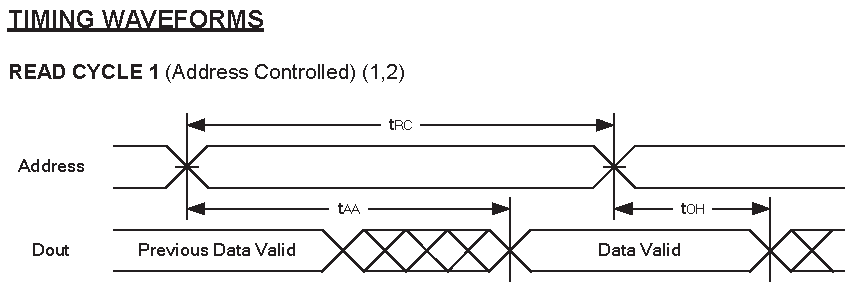
\includegraphics[width=\textwidth]{resources/read_cycle-rc.pdf}
	\caption{De typische lees cyclus van de SRAM chip \cite{ram-datasheet}}
	\label{fig:ramcontroller-read-cycle}
\end{figure}

\begin{figure}[H]
\centering
	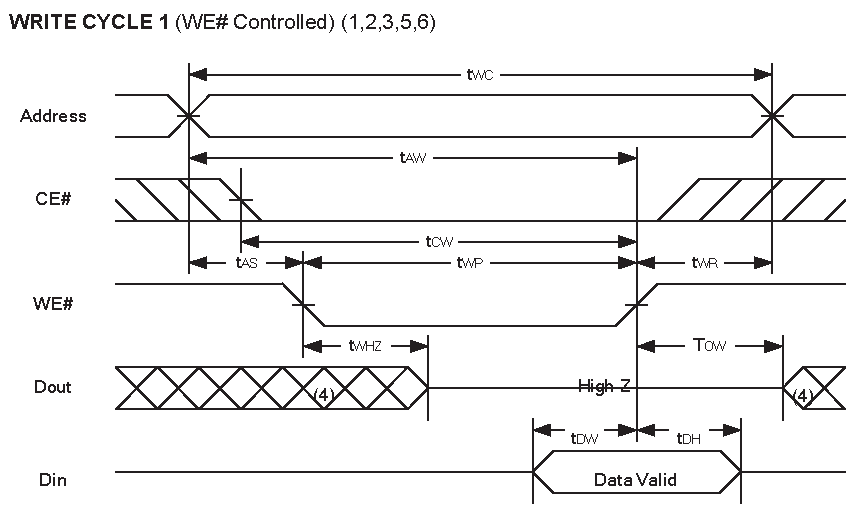
\includegraphics[width=\textwidth]{resources/write_cycle-rc.pdf}
	\caption{De typische schrijf cyclus van de SRAM chip \cite{ram-datasheet}}
	\label{fig:ramcontroller-write-cycle}
\end{figure}

\begin{figure}[H]
\centering
	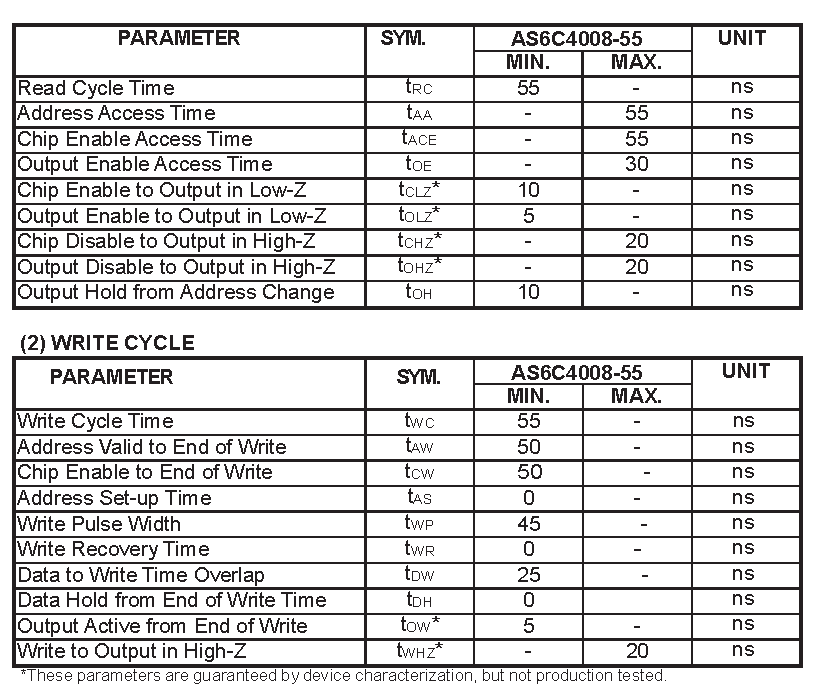
\includegraphics[width=\textwidth]{resources/time_constraints-rc.pdf}
	\caption{De “time-constraints” van de SRAM chip \cite{ram-datasheet}}
	\label{fig:ramcontroller-time-constraints}
\end{figure}

%VHDL Sim
\subsection{VHDL simulatie}
De VHDL is zeer kort en bondig. Het zorgt dat de uitgangen voldoen aan de waarheidstabellen.
In de simulatie zien we dat inderdaad de waarheidstabel goed geimplementeerd is.

\begin{figure}[H]
\centering
	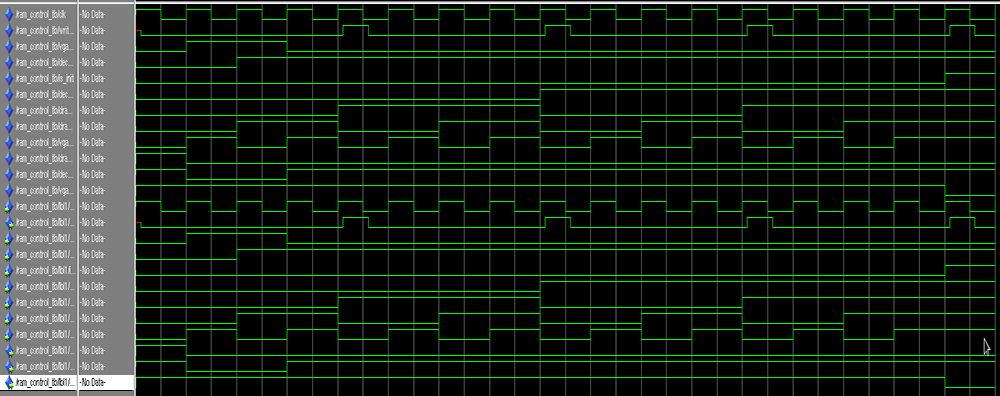
\includegraphics[width=\textwidth]{resources/wave-narrow.png}
	\caption{Het resultaat van de ModelSim-simulatie}
	\label{fig:ramcontroller-sim}
\end{figure}

%Synthese
\subsection{Synthese \& Layout}
Zoals te zien in in de layout (Figuur \ref{fig:ramcontroller-layout}) is dit een zeer compacte module. De simulaties in modelsim van de extracted en sythesized VHDL geven één zelfde beeld.

\begin{figure}[H]
\centering
	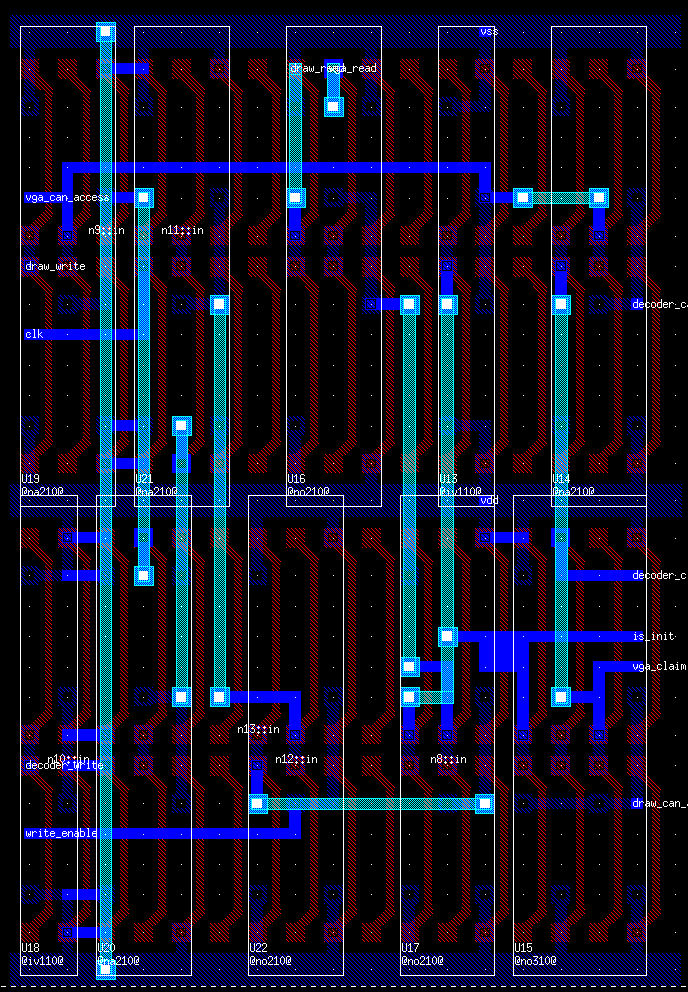
\includegraphics[width=0.5\textwidth]{resources/layout_ramcontroller.png}
	\caption{De RAM controller layout}
	\label{fig:ramcontroller-layout}
\end{figure}

%Switchlevel test
\subsection{Switchlevel}
De switch level simulatie verliep vlekkeloos. Zie Figuur \ref{fig:ramcontroller-sl-sim}.
\begin{figure}[H]
\centering
	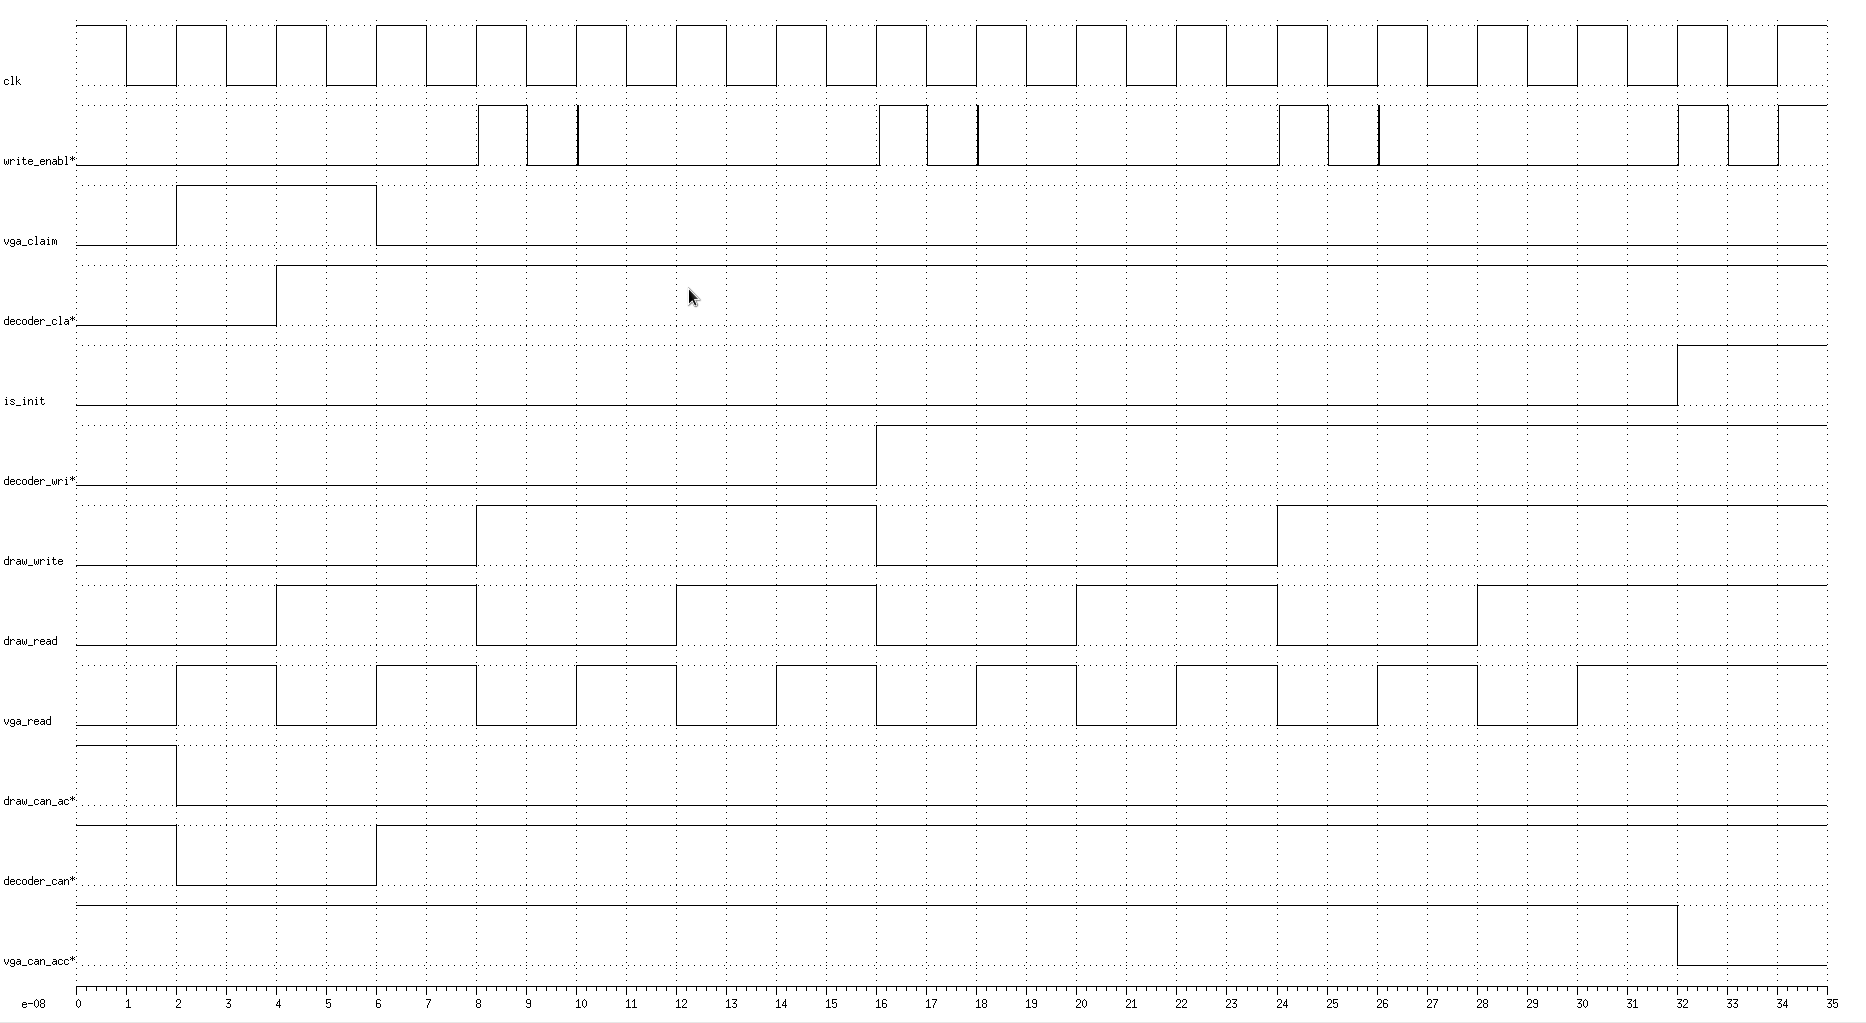
\includegraphics[width=0.5\textwidth]{resources/wave_sls.png}
	\caption{De RAM controller layout}
	\label{fig:ramcontroller-sl-sim}
\end{figure}

%Conclusie
\subsection{Conclusie}
Als we de resultaten van de SLS simulatie vergelijken met de resultaten uit modelsim dan komen die exact overeen.

\end{document}